\documentclass[12pt]{article}
\usepackage[utf8]{inputenc}

\title{Analysis of the Traveling Salesman Problem}
\author{Benny Chen}
\date{\today}

\usepackage{color}
\usepackage{amsthm}
\usepackage{amssymb} 
\usepackage{amsmath}
\usepackage{listings}
\usepackage{xcolor}
\usepackage{listings}
\usepackage{graphicx}
\usepackage{subcaption}
\usepackage{caption}
\usepackage{tikz}
\usepackage{pgfplots}
\usepackage{pgfplotstable}
\usepackage[hidelinks]{hyperref}

\newtheorem{Definition}{Definition}
\newtheorem{algorithm}{Algorithm}
\begin{document}


\maketitle

\section{Introduction}
Back in the 1800s, the mathematician Thomas Penyngton Kirkman posed the following problem: Given a list of $n$ cities and the distances between each pair of cities, what is the shortest possible route that visits each city exactly once and returns to the origin city? This problem is known as the \textit{Traveling Salesman Problem}. The problem is named after the salesman who must travel between cities to sell his goods. The salesman must travel between cities in a way that minimizes the total distance traveled. There are many variations and extensions of the problem, but the original problem is the most well-known. For example, in the 1930s, mathematician Merrill Flood tried to solve the problem of finding the shortest route for school buses. This however leads him to consider the problem 
mathematically. This problem became extremely popular in the 1950s with multiple prizes and incentives being offered for a solution. The problem now has many solutions, with each solution having its advantages and disadvantages and are still being improved upon today. In this paper, we will analyze the problem and some of its solutions.

\begin{center}
    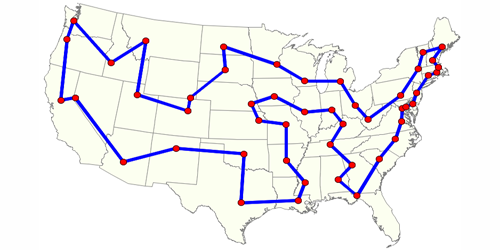
\includegraphics[scale = .5]{images/graph2.png}
\end{center}

\section{Definitions}
\subsection*{Graphs}
\begin{Definition}
A graph is a set of vertices and edges. A vertex is a point in the graph and an edge is a line connecting two vertices. Edges can be weighted, which means that each edge has a value associated with it or the cost of traveling along that edge.
\end{Definition}

\subsection*{Complete Graph}
\begin{Definition}
A complete graph is a graph where every vertex is connected to every other vertex.
\end{Definition}

\subsection*{Hamiltonian Cycle}
\begin{Definition}
A Hamiltonian cycle is a cycle that visits every vertex exactly once and ends on the first vertex.
\end{Definition}

\subsection*{Hamiltonian Path}
\begin{Definition}
A Hamiltonian path is a path that visits every vertex exactly once but does not end on the first vertex.
\end{Definition}

\section{NP-Completeness}
The Traveling Salesman Problem is an NP-Complete problem. An NP problem is a problem that is a set of decision problems that are making yes/no decisions. Another criteria for an NP problem is that the problem can be verified in polynomial time. An NP-Complete problem is an NP problem that can be reduced down to be able to solve any other NP problem. By categorizing the Traveling Salesman Problem as an NP-Complete problem, it means that the problem is very difficult to solve and does not have a truly efficient solution yet. This means that if someone were to find the most efficient solution to the problem, they would be able to solve any other NP problem. 

\begin{center}
    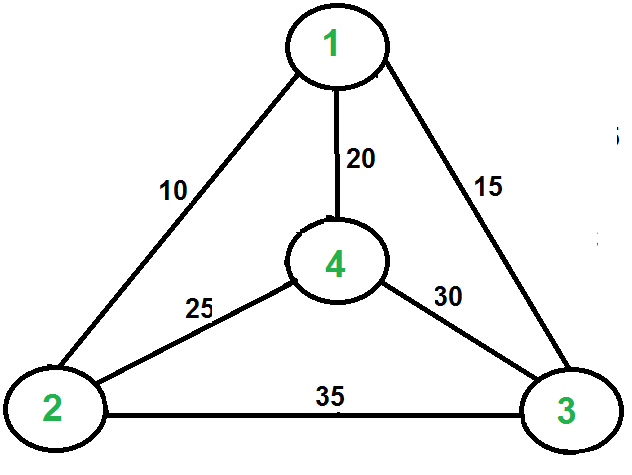
\includegraphics[scale = .5]{images/graph1.png}
\end{center}

\section{Solutions}
There are many solutions to the Traveling Salesman Problem and even more solutions are currently being developed. The most popular solution is brute force, which is a solution that tries every possible Hamiltonian cycle and returns the one with the minimum total weight. This solution
is very slow and is not practical for large graphs. Another solution is
the Nearest Neighbor algorithm, which is a greedy algorithm that starts
at a vertex and then visits the nearest vertex that has not been visited
yet. This solution is again also not practical for large graphs.

\subsection{Brute Force}
The brute force solution is a solution that tries every possible Hamiltonian
cycle and returns the one with the minimum total weight. This solution
is very slow and is not practical for large graphs. The brute force solution
can be implemented using recursion. The algorithm will start at the first
vertex and then try every possible Hamiltonian path that starts at that
vertex. The algorithm will then return the Hamiltonian path with the minimum
total weight. This is by far the slowest solution to the problem, however
it is the most straightforward solution. This method would run factorially
as the number of vertices increases. This means that the time complexity
of the algorithm is $O(n!)$. 

\begin{center}
    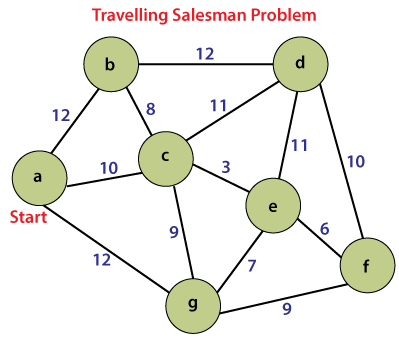
\includegraphics[scale = .5]{images/graph3.png}
\end{center}

\subsection{Nearest Neighbor}
The Nearest Neighbor algorithm is a greedy algorithm which is a algorithm
that makes the best or ``greedy'' choice at each step. The Nearest Neighbor algorithm is very simple, it starts at any vertex and then visits the nearest connecting vertex that has
not been visited yet with the least cost or weight. At the end of the algorithm, it will return a Hamiltonian Path of the minimum total weight. This algorithm is also not practical for large graphs as when the number of vertices increases, the time complexity increases exponentially. This means that the time complexity of the algorithm is $O(n^2)$.

\subsection{Held-Karp}
To this day, there is not a unanimous solution to the Traveling Salesman Problem. Many people around the world have taken on the challenge along with trying to solve other variations of the problem. The most popular solution today and known as the most efficient and optimal solution is the Held-Karp algorithm. This algorithm is a dynamic programming algorithm that uses a table to store the minimum weight of a Hamiltonian Path that starts at a vertex and ends at a vertex. By doing this, the algorithm can look up the minimum weight of a Hamiltonian Path in the table instead of having to calculate it. 

\section{Present Day}
The Traveling Salesman Problem is still being studied and improved upon today. There are many solutions to the problem and many more solutions are being developed. Even though there is no unanimous solution to the problem, many companies and people use the problem in real life. For example, one of the biggest applications in the world, Google Maps, uses a form of the Traveling Salesman Problem to find the shortest route between two points. It uses another algorithm called dijkstra's algorithm to find the shortest route between two points. The Traveling Salesman Problem appears in many other applications such as the scheduling of flights and electronic circuit design. By being able to route different paths on a map, we can create more efficient routes and save time and money. With more and more solutions being developed, we can expect to see the problem becoming more and more efficient and practical.

\nocite{*}
\bibliographystyle{plain}
\bibliography{sources.bib}

\end{document}
